\chapter[Método]{Método}

O método utilizado é uma interpretação do processo para descoberta de conhecimento proposto por \citeonline{fayyad1996data}, onde o objetivo principal é mapear um grande volume de dados para formas mais compactas, abstratas ou úteis para se encontrar padrões\footnote{O termo padrão é utilizado neste trabalho para designar um padrão encontrado nos dados.} e extrair informação.

A \autoref{fig:processo} apresenta o processo no qual, a partir de um conjunto de currículos Lattes, são obtidos indicadores em redes de coautoria inter- e intra-áreas que são analisados para determinar o impacto que uma área do conhecimento exerce em outra.

\begin{figure}[htpb]
  \centering
  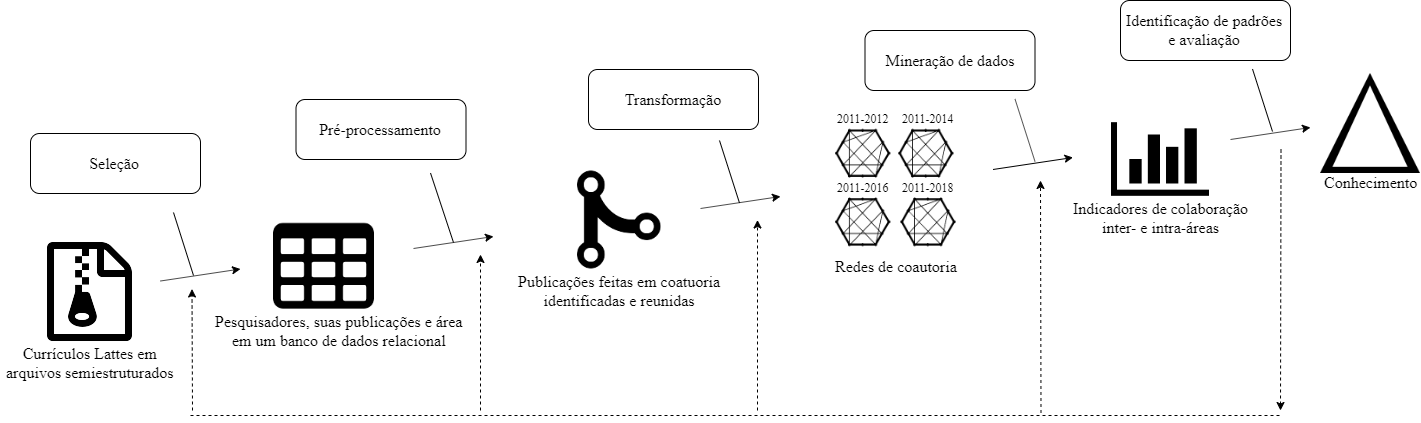
\includegraphics[width=1\textwidth]{figuras/metodo-diagrama-fayyad}
  \caption{Uma visão geral das etapas adotadas no processo de descoberta de conhecimento.}
  \label{fig:processo}
\end{figure}

As etapas de seleção, pré-processamento e transformação preparam o conjunto de dados para a etapa de mineração de dados, onde são aplicados algoritmos para extrair padrões. Esses padrões são então interpretados e utilizados para gerar conhecimento.

\section{Seleção}

Os currículos Lattes em formato XML foram processados por um sistema\footnote{Foram construídos dois programas. No primeiro, os atributos do currículo especificados são recuperados e armazenados intermediariamente em um arquivo no formato JSON. O segundo usa esse arquivo intermediário para fazer a carga nas tabelas do banco de dados remoto. Isso foi feito para evitar que a interpretação dos arquivos estivesse sujeita a instabilidades na conexão de rede e fosse possível continuar o processamento sem perdas em caso de falha.} onde as áreas de atuação do pesquisador e sua produção bibliográfica foram extraídas e armazenadas em um banco de dados relacional.

A \autoref{fig:er} apresenta a modelagem de dados lógica do currículo Lattes centrada nos atributos que são de interesse para este trabalho, a qual descreve os pesquisadores atuando em múltiplas áreas do conhecimento e escrevendo múltiplas publicações científicas. O modelo físico do banco de dados está representado no \autoref{ap:diagramacurriculo}.

\begin{figure}[htpb]
  \centering
  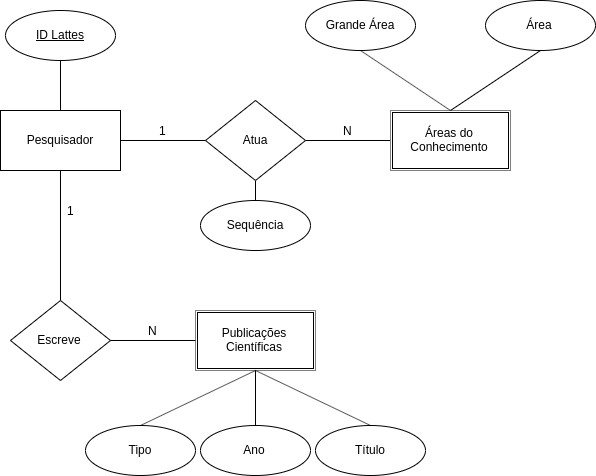
\includegraphics[scale=.5]{figuras/metodo-modelo-logico-lattes}
  \caption{Modelo entidade-relacionamento lógico descrevendo as relações entre o pesquisador, suas áreas de atuação e suas publicações científicas.}
  \label{fig:er}
\end{figure}

\section{Pré-processamento}

\subsection{Normalização do título das publicações}

Diversas produções científicas nessa área \cite{franceschet2011collaboration} \cite{mena2013prospecccao} \cite{reuther2006managing} descrevem casos onde uma publicação têm diversos nomes (sinônimos) e casos onde diferentes publicações possuem o mesmo nome (homônimos), cujos requerem tratamento a fim de obter um resultado mais confiável na etapa seguinte.

Publicações sinônimas acontecem neste trabalho porque os autores não cadastraram o título da publicação exatamente da mesma maneira. Existem casos onde há abreviação de palavras, omissão de pontuação ou erros de digitação, por exemplo. Ainda, foram encontrados casos onde existem metadados para formatação do título, como itálico e negrito, que são colocados por alguns autores.

Assim, o \autoref{alg:normalizacao} foi proposto para normalizar o título das publicações removendo diacríticos\footnote{Um diacrítico é um sinal gráfico que se coloca sobre, sob ou através de uma letra para alterar a sua realização fonética ou marcar qualquer outra característica linguística.}, espaços em branco e metadados de formatação ou qualquer outro elemento de marcação. Antes dessa etapa, podiam ser identificadas $1.230.082$ coautorias considerando o título exato e o ano da publicação. Após o pré-processamento, o número foi para $1.564.737$, o que já se traduz em uma melhora de $27$\% na identificação de coautorias.

\begin{algorithm}
  \caption{Normalização do título das publicações}
  \label{alg:normalizacao}
  \begin{algorithmic}[1]
  \Procedure{NormalizeTitulo}{titulo}
    \State $titulo\gets \Call{UnescapeHtml}{titulo}$ \Comment{Remove codificação HTML-safe}
    \If{$titulo$ contém o termo CDATA entre colchetes}
        \State $titulo\gets$ conteúdo do CDATA
    \EndIf
    \If{$titulo$ contém fragmentos que começam com $<$ e terminam com $>$}
        \State $titulo\gets titulo$ sem os fragmentos  
    \EndIf
    \State $titulo\gets \Call{NormalizeParaFormaNFKD}{titulo}$
    \State $resultado\gets \emptyset$
    \State $mantenha_{diacritico}\gets Falso$
    \ForAll{$c \in titulo$}
        \If{$c$ não é branco \textbf{and} $c$ não é um diacrítico \textbf{or} $mantenha_{diacritico}$}
            \State $resultado \gets resultado \cup \{c\}$
            \If{$c$ é um símbolo ASCII}
                \State $mantenha_{diacritico}\gets Falso$
            \Else
                \State $mantenha_{diacritico}\gets Verdadeiro$
            \EndIf
        \EndIf
    \EndFor
    \State $titulo\gets resultado$
    \State $titulo\gets \Call{NormalizeParaFormaNFC}{titulo}$
    \State \Return $titulo$
  \EndProcedure
  \end{algorithmic}
\end{algorithm}

Assume-se que publicações homônimas são mais difíceis de ocorrer dado que as coautorias serão identificadas apenas para publicações de um mesmo tipo em um mesmo ano, e por isso nenhum tratamento foi realizado. Porém, caso publicações homônimas existam nesse conjunto de dados, seria possível observar que a lista de coautores de um autor se dividiria em dois ou mais grupos altamente interconectados, sem colaborações entre os grupos diferentes \cite{franceschet2011collaboration}.

\subsection{Identificação da área de atuação do pesquisador}

As coautorias entre as áreas do conhecimento podem ser observadas se as áreas do conhecimento na qual o pesquisador 

Uma forma de fazer a leitura de como as coautorias acontecem entre as diferentes áreas do conhecimento é atribuindo a cada um dos coautores sua  rotular a qual área do conhecimento cada pesquisador mais se encaixa. Isso faz com que seja necessária a definição de um método para escolher uma área dentre todas as presentes no currículo.

O \autoref{alg:identificacaoarea} foi construído de tal forma que a área mais frequente será selecionada na maioria dos casos, a única exceção acontece quando a área mais frequente não pertence à grande área que mais aparece no currículo, pois esta tem prioridade. Em casos de empate, a área que aparece com menor sequência, isto é, aparece primeiro no currículo, é selecionada uma vez que a ordenação é estável.

\begin{algorithm}
  \caption{Identificação da área de atuação do pesquisador}
  \label{alg:identificacaoarea}
  \begin{algorithmic}[1]
  \Procedure{IdentificaArea}{A}
    \State $areaIdentificada\gets \textbf{nulo}$
    \State $raiz\gets \Call{NoVazio}$
    \ForAll{$area \in A$}
        \State $grandeArea\gets \Call{GrandeArea}{area}$
        \State $area\gets \Call{Area}{area}$
        \State $no\gets \Call{RecuperaNo}{raiz, grandeArea}$
        \If {$no$ não existe}
            \State $no\gets \Call{IncluirNo}{raiz, grandeArea}$
        \EndIf
        \State $no.contagem++$
        \If{$area$ está preenchida}
            \State $folha\gets \Call{RecuperaNo}{no, area}$
            \If{$folha$ não existe}
                \State $folha\gets \Call{IncluirNo}{no, area}$
            \EndIf
            \State $folha.contagem++$
        \Else
            \State $no.contagemVazios++$
        \EndIf
    \EndFor
    \State $N\gets \Call{OrdenaPorContagem}{raiz.filhos, \textbf{decrescente}}$
    \While{$areaSelecionada \neq \textbf{nulo}$}
        \State $no\gets \Call{Proximo}{N}$
        \If{$no.contagem \neq no.contagemVazios$}
            \State $F\gets \Call{OrdenaPorContagem}{no.filhos, \textbf{decrescente}}$
            \State $areaSelecionada\gets \Call{Proximo}{F}$
        \EndIf
    \EndWhile
    \State \Return $areaSelecionada$
  \EndProcedure
  \end{algorithmic}
\end{algorithm}

\section{Transformação}

A partir das publicações científicas obtidas nos currículos é possível identificar dois pesquisadores como coautores se uma mesma publicação aparece em seus currículos. Com isso é possível construir uma rede de coautoria onde os nós são pesquisadores e os vértices a coautoria entre eles.

Sabendo que uma coautoria só deve ser identificada se as publicações forem do mesmo tipo e ano, mas que os títulos não precisam ser exatamente iguais, o \autoref{alg:coautoria} foi proposto para construir a lista de adjacência das redes de coautorias.

\begin{algorithm}
  \caption{Identificação de coautorias}
  \label{alg:coautoria}
  \begin{algorithmic}[1]
  \Procedure{IdentificaCoautoria}{P}
    \State $P^2\gets P\times{P}$
    \State $C\gets \emptyset$
    \ForAll{$(p_1, p_2) \in P^2$}
    \If{$\Call{Indice}{p_1} < \Call{Indice}{p_2}$}
      \State \textbf{next}
    \ElsIf{$\Call{Autor}{p_1} = \Call{Autor}{p_2}$}
      \State \textbf{next}
    \ElsIf{$\Call{Palavras}{p_1} \leq 2$ \textbf{or} $\Call{Palavras}{p_2} \leq 2$}
      \State \textbf{next}
    \Else
      \State $tamanho_{p1}\gets \Call{TamanhoDoTitulo}{p_1}$
      \State $tamanho_{p2}\gets \Call{TamanhoDoTitulo}{p_2}$
      \State $similaridade_{tam}\gets \dfrac{\min\{t_1, t_2\}}{\max\{t_1, t_2\}}$
      \If{$similaridade_{tam} \geq 0,9$}
        \State $distancia\gets \Call{DistanciaLevenshthein}{p_1, p_2}$
        \State $similaridade_{lev}\gets 1 - \dfrac{distancia}{\max\{t_1, t_2\}}$
        \If{$similaridade_{lev} \geq 0,9$}
            \State $C\gets C\cup\{(p1, p2)\}$
        \EndIf
      \EndIf
    \EndIf
    \EndFor
    \State $C\gets \Call{TransformaComponentesConexasEmCliques}{C}$
    \State \Return $C$
  \EndProcedure
  \end{algorithmic}
\end{algorithm}

Assim, em um conjunto de publicações do mesmo tipo e ano, as publicações com títulos que são pelo menos 90\% similares, de autores diferentes e títulos contendo pelo menos duas palavras, são identificas como uma coautoria. O cálculo da similaridade é feito a partir da distância de Levenshtein \cite{levenshtein1965binary}, que quantifica a dissimilaridade entre os títulos. A transformação das componentes conexas em cliques no final do procedimento garante que todos os coautores estejam relacionados entre si.

\section{Mineração de dados}

A partir dessa rede de colaboração entre as áreas foram construídas redes, tabelas e gráficos. Foram utilizadas medidas de diâmetro da rede, grau, caminho médio, coeficiente médio de clusterização, dentre outras, para caracterizar o impacto da Ciência da Computação.

Grande parte dos gráficos e tabelas apresentam a frequência com que as publicações ocorrem, dada uma condição. Uma exceção é o mapa de calor da \autoref{fig:mapadecalorcolaboracao}, onde cada linha representa as colaborações dessa área dividida pela maior colaboração, o que nos permite observar o quanto uma colaboração representa na produção bibliográfica feita em coautoria com relação às demais áreas.

\section{Identificação de padrões e avaliação}

Foi feita uma análise condicional dos dados, uma vez que são considerados apenas as publicações científicas que possuem ano preenchido cujos autores têm a área de atuação preenchida.

Por meio da análise dos gráficos e redes construídas, o impacto que a Ciência exerce nas demais áreas pôde ser avaliado.
